\large \emph{\textbf{Antton Cattarin}}

The first part of this project discusses the use of cubic spline interpolation. This algorithm was used to interpolate a series of points representing an airfoil. Between each point, the algorithm computed a polynomial with a degree at most 3. The final interpolation was a continuous function passing by all the points. This algorithm was implemented with the help of \emph{Numerical Recipes}. Figure \ref{fig:interp} below illustrates the results for known functions.

\begin{figure}[h]
  \centering
  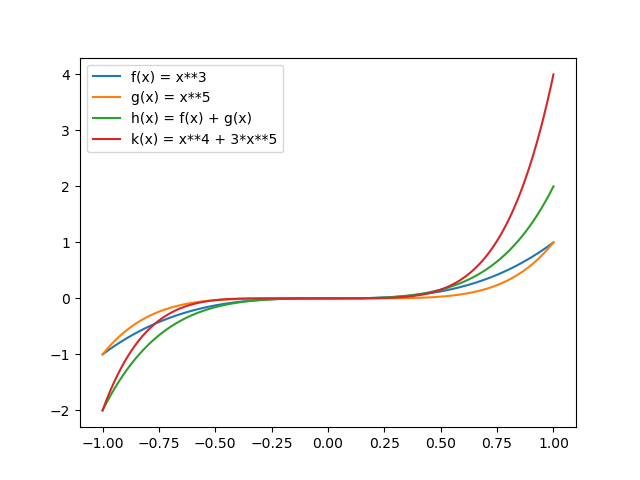
\includegraphics[width=0.45\textwidth]{img/interpolations.png}
  \caption{Cubic interpolations of known functions}
  \label{fig:interp}
\end{figure}

These results are visually significant as the curves look like the functions. This was also verified numerically.

\bigskip


Following that, the cubic spline algorithm was used to compute functions representing an airfoil. A series of points were given in a file. This algorithm was applied to these points, and a function was identified. This function and the points can be observed in Figure \ref{fig:airfoil}.

\begin{figure}[h]
  \centering
  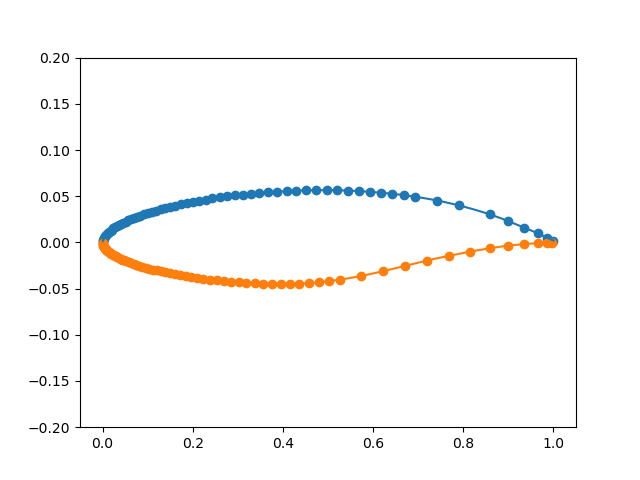
\includegraphics[width=0.45\textwidth]{img/airfoil_interp.png}
  \caption{Cubic interpolations of the airfoil}
  \label{fig:airfoil}
\end{figure}
  
This graph exhibits the links between all the points and the resultant function.

\bigskip

To use this algorithm, the boundary conditions were defined. Typically, the second derivatives at the first and last points are fixed at 0. In our implementation, the algorithm took the first derivatives and computed the second derivatives. To obtain the second derivatives equal to 0, the first derivatives had to be more than $10^{30}$.

The values of the first derivatives impacted the interpolation curves around the first and last points.
